\section{Measurements of the CKM angle $\beta$}
\label{sec:beta}

While the world average~\cite{HFAG} of $\beta$ is still dominated
by the BaBar and Belle measurements, LHCb also contributes~\cite{} and can be expected
to reach the BaBar and Belle individual sensitivities once Run~II data and
improvements in flavour tagging are included in the analysis. LHCb has also measured~\cite{}
$CP$ violation in $B^0_s \to J/\psi K^0_S$ decays,
which can help to constrain the size of penguin contributions to the measurement
of $\beta$ from $B^0 \to J/\psi K^0_S$, as well as the $CP$ violating parameters in
$B^0 \to D^+ D^-$ decays, which can also be interepreted in terms of constraints on $\beta$.
The current world average of measurements of $B^0 \to D^+ D^-$ is shown in Fig.~\ref{b2ddwa}, 
interestingly while all measurements are compatible with each other, the LHCb measurement
does not confirm the maximal (within uncertainty) Belle measurement of $S$.

\begin{figure}
  \begin{center}
    \begin{tabular}{c c}
      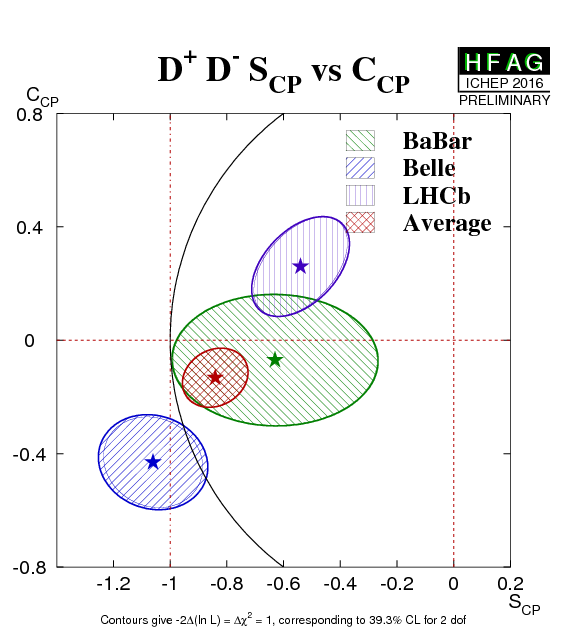
\includegraphics[height=7.5cm]{figs/D+D-S_CPvsC_CP.png} &
    \end{tabular}
  \end{center}
  \vspace{-0.5cm}
  \caption{\label{b2ddwa}World average of time-dependent $CP$ observables in $B^0 \to D^+ D^-$, reproduced from HFAG~\cite{HFAG}.}
\end{figure}

The BaBar and Belle Collaboration obtained the first observation of $CP$-violation
in the channels $B^0 \to D^{(*)}_{CP} h^0$, where $h^0$ is a light unflavored neutral
meson, by combining their final datasets \cite{babar_belle_D0h0}. Neglecting the
very small contribution from the $CKM$ suppressed amplitude $b \to u\bar{c}d$,
the time dependent analysis is sensitive to $\sin(2\beta)$. A joint likelihood,
sharing the same physics parameters but independent background modeling parameters,
the two experiments find:
\begin{eqnarray}
-\eta_f S & = & +0.66 \pm 0.10 (\mbox{stat}) \pm 0.16 (\mbox{syst}), \\
C & = & +0.02 \pm 0.07 (\mbox{stat}) \pm 0.03 (\mbox{syst}), 
\end{eqnarray}
with the significance of the observation beeing 5.4 standard deviations. 
